% !TeX TS-program = xelatex

\documentclass[]{beamer}
%\usefonttheme[onlymath]{serif}

%Set the slide theme
%Change to meet your taste
% Madrid, Copenhagen, Berlin, ... works
%\usetheme{Copenhagen} 

%\usetheme{Antibes}
\usetheme{Ilmenau}
\usepackage{graphicx}
\usepackage{xecolor}
\usepackage{amsmath}
%\usefonttheme[onlymath]{sanserif} %Change the math font
\usepackage{bm}
\newtheorem{den}{{\large\bf تعریف}}[section]
\newtheorem{exa}{{\large\bf مثال}}[section]
\newtheorem{lem}{{\large\bf لم}}[section]
\newtheorem{pro}{{\large\bf گزاره}}[section]
\newtheorem{cor}{{\large\bf نتیجه}}[section]
\newtheorem{thm}{{\large\bf قضیه}}[section]
\newtheorem{rem}{{\large\bf تذکر}}[section]
\newtheorem{nnt}{{\large\bf توجه}}[section]
\usepackage {tikz}
\usetikzlibrary {positioning}
\usetikzlibrary{decorations.pathreplacing}
\usepackage[framemethod=tikz]{mdframed}


\usetikzlibrary{decorations.markings}

\tikzset{
	tangent/.style={
		decoration={
			markings,% switch on markings
			mark=
			at position #1
			with
			{
				\coordinate (tangent point-\pgfkeysvalueof{/pgf/decoration/mark info/sequence number}) at (0pt,0pt);
				\coordinate (tangent unit vector-\pgfkeysvalueof{/pgf/decoration/mark info/sequence number}) at (1,0pt);
				\coordinate (tangent orthogonal unit vector-\pgfkeysvalueof{/pgf/decoration/mark info/sequence number}) at (0pt,1);
			}
		},
		postaction=decorate
	},
	use tangent/.style={
		shift=(tangent point-#1),
		x=(tangent unit vector-#1),
		y=(tangent orthogonal unit vector-#1)
	},
	use tangent/.default=1
}

\usepackage{xepersian}
\settextfont{XB Niloofar}
%\DefaultMathsDigits



\newcommand{\bfphi}{\mathbf{\phi}}
\newcommand{\E}{\mathbb{E}}
\newcommand{\N}{\mathcal{N}}
\newcommand{\Prob}{\mathbb{P}}
%\newcommand{\bfphi}{{\pmb \phi}}
%\newcommand{\bfphi}{\bm \phi}
\newcommand{\mubf}{\bm \mu}
\newcommand{\Ybf}{\bm Y}
\newcommand{\Hc}{\mathcal{H}}
\newcommand{\bx}{\mathbf{x}}
\newcommand{\R}{\mathbb{R}}
\newcommand{\Nd}{\mathcal{N}}
\newcommand{\tr}{\mathrm{tr}}
\newcommand{\HSIC}{\mathrm{HSIC}}
\newcommand{\LL}{\mathcal{L}}
\newcommand{\bigCI}{\mathrel{\text{\scalebox{1.07}{$\perp\mkern-10mu\perp$}}}}
%---------------------------------------------------------------------------------
% Seetings to force Beamer works with Xepersian and RTL typesetting
%-------------------------------------------------------------------------------
%\raggedleft

% For right to left lists (itemize and enumerate)
\makeatletter

\newcommand{ \RTList}{\raggedleft\rightskip\@totalleftmargin} 

\makeatother
\defbeamertemplate*{footline}{shadow theme}
{%
	\leavevmode%
	\hbox{\begin{beamercolorbox}[wd=.5\paperwidth,ht=2.5ex,dp=1.125ex,leftskip=.3cm plus1fil,rightskip=.3cm]{author in head/foot}%
			\usebeamerfont{author in head/foot}\insertframenumber\,/\,\inserttotalframenumber\hfill\insertshortauthor
		\end{beamercolorbox}%
		\begin{beamercolorbox}[wd=.5\paperwidth,ht=2.5ex,dp=1.125ex,leftskip=.3cm,rightskip=.3cm plus1fil]{title in head/foot}%
			\usebeamerfont{title in head/foot}\insertshorttitle%
	\end{beamercolorbox}}%
	\vskip0pt%
}
% Correct the bullet for RTL texts
\setbeamertemplate{itemize item}{\scriptsize\raise1.25pt%
 \hbox{\donotcoloroutermaths$\blacktriangleleft$}} 

% To force beamer use numbering in captions
\setbeamertemplate{caption}[numbered]{}% Number float-like environments


\renewcommand{\familydefault}{\sfdefault}
%---------------------------------------------------------------------------------
\title[کنترل‌کردن سوییدگی در استفاده کردن از اطّلاعات]{
کنترل‌کردن سوییدگی در استفاده کردن از اطّلاعات\\
\small{
ارائه‌ی پروژه‌ی درس تئوری اطّلاعات}}

\author[بهراد منیری
و محمّدرضا رحمانی
]{
	بهراد منیری
\and
	محمّدرضا رحمانی\\
		\vspace{0.5cm}
	\scriptsize استاد درس\\
	\small
	دکتر  میرمحسنی\\
	\vspace{0.5cm}
	\scriptsize
	 دستیار آموزشی\\ 
	 \small
	 امیرحسین بساره
}


\institute[دانشگاه‌ صنعتی شریف]{
دانشکده‌ی مهندسی برق\\
دانشگاه صنعتی شریف
}


\date{}


\begin{document}
\begin{persian}
%------------------------------------------
% Title page
%------------------------------------------
\begin{frame}
\maketitle
\end{frame}

% To adjust the paragraphs in RTL
\everypar{\rightskip\rightmargin}
%-------------------------------------------------------------------------------

\begin{frame}
\frametitle{فهرست}
\tableofcontents
\end{frame}

\section{معرفی}

\begin{frame}
\begin{center}
	\begin{latin}
	\Large{How much does your data exploration overfit? Controlling bias via information usage}\\
	\vspace{0.6cm}
	\large{Daniel Russo$^1$, James Zou$^2$}\\
	\vspace{0.3cm}
	\normalsize{IEEE Transactions on Information Theory, 2019}\\	
	\vspace{1cm}
	\small{
	$^1$The  Division  of  Decision,  Risk  and  Operations, Columbia University\\
	$^2$Biomedical Data Science, Computer Science and Electrical Engineering at Stanford University
}

	\end{latin}
\end{center}
\end{frame}


\section{انگیزه}
\begin{frame}
\begin{figure}[h!]
	\frametitle{انگیزه}
	\centering
	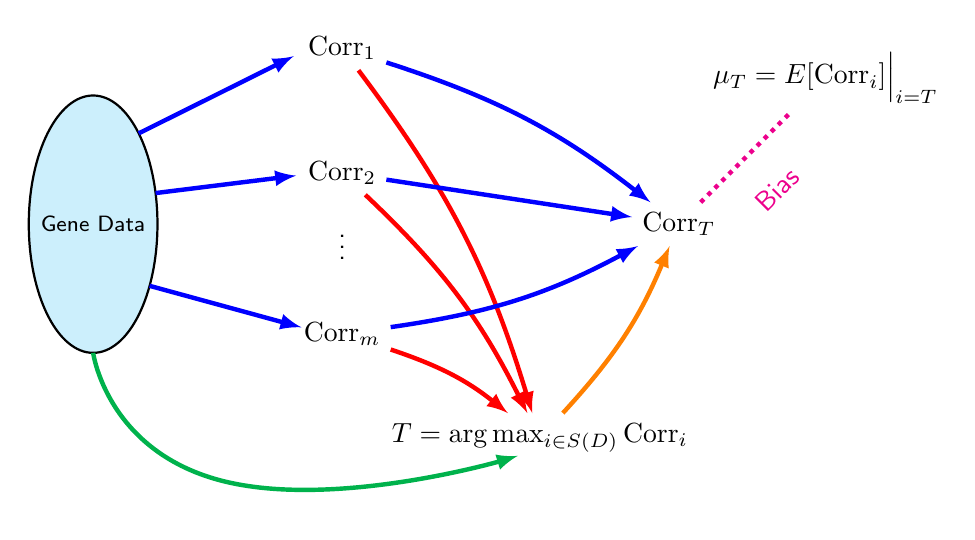
\begin{tikzpicture}[auto, node distance=0.5cm, every loop/.style={},
	thick,state/.style={font=\sffamily\Large}, scale = 0.93]
	
	\onslide<1->{
	\filldraw[fill=cyan!20!white, tangent=0.15, tangent=0.05,  tangent=-0.1, tangent=-0.2](0, 0) ellipse (25pt and 50pt);
	\node[state] (data) {\footnotesize Gene Data};
	%	    \draw (0,0) ellipse (1cm and 2cm);
	
	
	}

	\onslide<2->{
	\node (phi1) at (3.4, +2.4) {$\mathrm{Corr}_1$} ;
	\node (phi2) at (3.4, 0.7) {$\mathrm{Corr}_2$} ;
	\node (phi3) at (3.4, -0.2) {$\vdots$} ;
	\node (phi4) at (3.4, -1.5) {$\mathrm{Corr}_m$} ;
	
	\draw [blue, ultra thick, use tangent, -latex] (0,0) -- (0,-2.2) node [pos=0.5, anchor=east] {};
	
	\draw [blue, ultra thick, use tangent=2, -latex] (0,0) -- (0,-1.8) node [pos=0.5, anchor=east] {};
	
	\draw [blue, ultra thick, use tangent=3, -latex] (0,0) -- (0,-2) node [pos=0.5, anchor=east] {};
	
	}
	\onslide<3->{

	\draw [green!70!blue, ultra thick, -latex] plot [smooth, tension=1] coordinates {(0,-50pt) (1.8,-100pt) (5.8,-90pt) };
	
	\node (T) at (6.1, -83pt) {$T = \arg\max_{i \in S(D)} \mathrm{Corr}_i$} ;
	
	
	\path [red, ultra thick]  (phi1) edge [bend left = 10, -latex] node[below =0.15 cm] {}(T);
	\path [red, ultra thick]  (phi2) edge [bend left = 10, -latex] node[below =0.15 cm] {}(T);
	\path [red, ultra thick]  (phi4) edge [bend left = 10, -latex] node[below =0.15 cm] {}(T);

	
}

\onslide<4->{
\node (final) at (8, 0) {$\mathrm{Corr}_T$} ;	

	\path [orange, ultra thick]  (T) edge [bend left = -10, -latex] node[below =0.15 cm] {}(final);


\path [blue, ultra thick] (phi1) edge [bend left = 10, -latex] node[below =0.15 cm] {}(final);
\path [blue, ultra thick]  (phi2) edge [bend left = 0, -latex] node[below =0.15 cm] {}(final);
\path [blue, ultra thick]  (phi4) edge [bend left = -10, -latex] node[below =0.15 cm] {}(final);

}

\onslide<5->{
\node (finalf) at (10, 2) {$\mu_T = \E [\mathrm{Corr}_i]\Big|_{i = T}$} ;	
\path [magenta, ultra thick, sloped] (final) edge [bend left = 0,  dotted] node[below =0.3 cm] {Bias}(finalf);

}
	\end{tikzpicture}
\end{figure}

\end{frame}

\begin{frame}
\begin{figure}[h!]
	\frametitle{انگیزه}
	\centering
	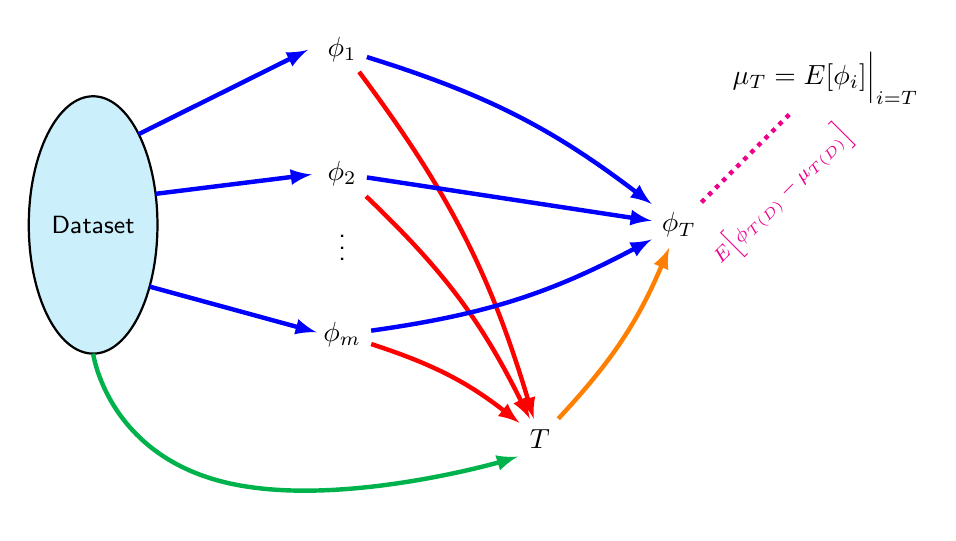
\begin{tikzpicture}[auto, node distance=0.5cm, every loop/.style={},
	thick,state/.style={font=\sffamily\Large}, scale = 0.93]

	\filldraw[fill=cyan!20!white, tangent=0.15, tangent=0.05,  tangent=-0.1, tangent=-0.2](0, 0) ellipse (25pt and 50pt);
	\node[state] (data) {\small Dataset};
%	    \draw (0,0) ellipse (1cm and 2cm);

	\node (phi1) at (3.4, +2.4) {$\phi_1$} ;
	\node (phi2) at (3.4, 0.7) {$\phi_2$} ;
	\node (phi3) at (3.4, -0.2) {$\vdots$} ;
	\node (phi4) at (3.4, -1.5) {$\phi_m$} ;

	\draw [blue, ultra thick, use tangent, -latex] (0,0) -- (0,-2.4) node [pos=0.5, anchor=east] {};
	
	\draw [blue, ultra thick, use tangent=2, -latex] (0,0) -- (0,-2) node [pos=0.5, anchor=east] {};
	
	\draw [blue, ultra thick, use tangent=3, -latex] (0,0) -- (0,-2.2) node [pos=0.5, anchor=east] {};



	\node (T) at (6.1, -83pt) {$T$} ;
	
		
	\path [red, ultra thick]  (phi1) edge [bend left = 10, -latex] node[below =0.15 cm] {}(T);
	\path [red, ultra thick]  (phi2) edge [bend left = 10, -latex] node[below =0.15 cm] {}(T);
	\path [red, ultra thick]  (phi4) edge [bend left = 10, -latex] node[below =0.15 cm] {}(T);

	\draw [green!70!blue, ultra thick, -latex] plot [smooth, tension=1] coordinates {(0,-50pt) (1.8,-100pt) (5.8,-90pt) };

	\node (final) at (8, 0) {$\phi_T$} ;
		\path [orange, ultra thick]  (T) edge [bend left = -10, -latex] node[below =0.15 cm] {}(final);	
	\path [blue, ultra thick] (phi1) edge [bend left = 10, -latex] node[below =0.15 cm] {}(final);
	\path [blue, ultra thick]  (phi2) edge [bend left = 0, -latex] node[below =0.15 cm] {}(final);
	\path [blue, ultra thick]  (phi4) edge [bend left = -10, -latex] node[below =0.15 cm] {}(final);


\node (finalf) at (10, 2) {$\mu_T = \E [\phi_i]\Big|_{i = T}$} ;	

\path [magenta, ultra thick, sloped] (final) edge [bend left = 0,  dotted] node[below =0.3 cm] {\scriptsize$\mathbb{E} \Big[ \phi_{T(D)} - \mu_{T(D)}\Big]$}(finalf);


	\end{tikzpicture}
\end{figure}

\end{frame}


\section{مدل ریاضی}




\begin{frame}



{
	\setbeamercolor{block title}{use=example text,fg=white,bg=example text.fg!75!black}
	\setbeamercolor{block body}{parent=normal text,use=block title example,bg=block title example.bg!10!bg}
\begin{thm}
	متغیّر تصادفی برداری
	\lr{$\bm{\phi} = (\phi_1,\cdots,\phi_m)$}
	را در نظر بگیرید، اگر تعریف کنیم
	\[\bm{\mu} = (\mu_1,\mu_2,\cdots,\mu_m)=\E[\bm{\phi}]\]
	و اگر برای هر
	\lr{$i\in\{1,\cdots,m\}$}،
	\lr{$\phi_i - \mu_i$}
	یک متغیّر تصادفی زیرگاوسی با پارامتر
	\lr{$\sigma$}
	باشد، آن‌گاه:
	\begin{equation}
	\Big|\E[\phi_T-\mu_T]\Big|\leq \sigma\sqrt{2I\,(T;\bm{\phi})}
	\end{equation}
	\begin{equation}
	\E\Big[\big|\phi_T-\mu_T\big|\Big]\leq \sigma + 36\sigma\sqrt{2I\,(T;\bm{\phi})}
	\end{equation}
	\begin{equation}
	\E\left[(\phi_T-\mu_T)^2\right]\leq 1.25\sigma^2 + 10\sigma^2I\,(T;\bm{\phi})
	\end{equation}

\end{thm}
}
\end{frame}



\section{کابرد‌های چهارچوب معرفی شده}
\begin{frame}
\frametitle{رتبه‌بندی با وجود سیگنال در داده‌ها}
\noindent
\begin{minipage}[t]{0.48\linewidth}
\begin{itemize}\RTList
	\item
	مدل تولید داده‌ها:
	\hspace{1.2cm}
	\hfill
	\begin{equation*}
	\phi_i \sim
	\begin{cases}
	\mathcal{N}(\mu, \sigma^2)\;\;\; i = I^{\;*}\\
	\mathcal{N}(0, \sigma^2)\;\;\; i \neq I^{\;*}
	\end{cases}
	\end{equation*}
	\item
	انتخاب:
		$$T = \arg\max_{i} \; \phi_i$$
	\item
کران مبتنی بر آنتروپی:
	\hspace{0.3cm}
	$$I\,(T; \bm{\phi}) = H(T\,) \leq \log(m)$$
	
\end{itemize}
\end{minipage}%
\begin{minipage}[t]{0.5\linewidth}
\begin{figure}
	\includegraphics[scale=0.35]{fig_1.png}
\end{figure}
\end{minipage}
\end{frame}


\begin{frame}
\frametitle{تفکیک تقریباً مستقل داده‌های غیر
\lr{i.i.d.}
}

\begin{figure}[h!]
	\centering

	\begin{tikzpicture}[ node distance=0.3cm, every loop/.style={},
	thick,state/.style={font=\sffamily\Large\bfseries},
	decoration={brace,mirror,amplitude=7}
	]
	\node[state] (s1) {$s_{1_{\;}}$};
	\node (do1)  [right=of s1] {$\cdots$};
	\node[state] (sn1) [right=of do1] {$s_{n_1}$};
	\node[state] (sn1p) [right=of sn1] {$s_{n_1+1}$};
	\node (do2)  [right=of sn1p] {$\cdots$};
	\node[state] (sn2) [right=of do2] {$s_{n_2}$};
	\node[state] (sn2p) [right=of sn2] {$s_{\tiny{n_2+1}}$};
		\node (do3)  [right=of sn2p] {$\cdots$};
	\node[state] (s5) [right=of do3] {$s_{t_{\;}}$};

	\path (s1) edge [bend left = -0] node[below =0.15 cm] {}(do1);
	\path (do1) edge [bend right = -0] node[below =0.15 cm]  {}(sn1);
	\path (sn1) edge [bend left = -0] node[below =0.15 cm]  {}(sn1p);
	\path (sn1p) edge [bend left = -0] node[below =0.15 cm]  {}(do2);
	\path (do2) edge [bend right = -0] node[below =0.15 cm]  {}(sn2);
	\path (sn2) edge [bend right = -0] node[below =0.15 cm]  {}(sn2p);
	\path (sn2p) edge [bend right = -0] node[below =0.15 cm]  {}(do3);
	\path (do3) edge [bend right = -0] node[below =0.15 cm]  {}(s5);
	
    \draw [decorate] ([yshift=-5mm]s1.west) --node[below=3mm]
    {تحلیل انتخاب } ([yshift=-5mm]sn1.east);
	\draw [decorate] ([yshift=-5mm]sn2p.west) --node[below=3mm]{تخمین} ([yshift=-5mm]s5.east);
	\end{tikzpicture}
\end{figure}
\begin{equation*}
\forall \tau \in \mathbb{N} \;\;\;\; \max_s D \Big (\mathbf{P}(s_{\tau} = .| s_1 = s) || \pi \Big) \leq c_0 e^{- c_1 \tau}
\label{myineq}
\end{equation*}


$$T \leftarrow \{s_1, \dots, s_{n_1}\} - s_{n_1} -  s_{n_2+1} - \{s_{n_2 + 1}, \dots, s_t\} \rightarrow \bm{\phi} $$

\begin{flalign*}
I\,(T;\bm{\phi}) &\leq I\,(s_{n_1}; s_{n_2+1})\\
&\leq c_0 e^{-c_1 (n_2-n_1)}
\end{flalign*}
\end{frame}

\section{تصادفی‌سازی}

\begin{frame}
\frametitle{انتخاب تصادفی اندیس}

\begin{itemize}\RTList
\item
چرا تصادفی‌سازی خوب است؟
$$I\,(T; \bm {\phi}) = H(T\,) - H(T\,|\bm{\phi}) = H\,(T\,) - H\,(\pi\,)$$

\item
در مسئله‌ی انتخاب ماکزیمم چه می‌توان کرد؟
	\begin{eqnarray*}
\underset{{ \pi} \in \mathbb{R}^m_+}{\text{maximize}} && H({\pi}) \\
\text{to subject } && \sum_{i=1}^{k} \pi_i \phi_i \geq b \mbox{ and }  \sum_{i=1}^{k} \pi_i =1.
\end{eqnarray*}

پاسخ این مسئله‌ی بهینه‌سازی:
$$\pi^* = Ae^{\beta \phi_i}$$
\end{itemize}

\end{frame}




\begin{frame}
\frametitle{انتخاب تصادفی اندیس}
\begin{minipage}[t]{0.46\linewidth}
\begin{itemize}\RTList
	\item
	نحوه‌ی تولید داده‌ها:
	\hspace{0.3cm}
	\begin{equation*}
	\begin{cases}
	\mu_i = \mu & i\leq N_1\\
	\mu_i = 0 & N_1 \leq i \leq N
	\end{cases}
	\end{equation*}

		\textbf{سوییدگی}:
		 $$\frac{1}{K} \sum_{i = 1}^{K} \phi_{T_i} - \mu_{T_i}$$
		\textbf{دقّت:}
		$$\frac{\big|\{T_i:T_i\leq N_1\}\big|}{K}$$

	
\end{itemize}
\end{minipage}
\begin{minipage}[t]{0.53\linewidth}
\begin{figure}
\centering
\includegraphics[scale=0.33]{fig_3.png}
\end{figure}
\end{minipage}
\end{frame}



\begin{frame}
\frametitle{مدل تحلیل تطبیقی داده‌ها}
\begin{itemize}\RTList
	\item
	در قدم اول، تحلیل 
	$\phi_{T_1}$
انتخاب می‌شود. نتیجه‌ی این تحلیل 
	$Y_{T_1} \in \R$
است.
	\item
	در تکرار 
	$k$ ام:
	$$T_k = f\big(Y_{T_1}, Y_{T_2}, \dots, Y_{T_k-1}, T_1, \dots, T_{k-1}\big)\Rightarrow\phi_{T_k}\Rightarrow Y_{T_k}$$
\end{itemize}

{
	\setbeamercolor{block title}{use=example text,fg=white,bg=example text.fg!75!black}
	\setbeamercolor{block body}{parent=normal text,use=block title example,bg=block title example.bg!10!bg}
\begin{pro}
	سوییدگی 
	$Y_{T_k}$
	دو جزء دارد:
\begin{align*}
&\E[|Y_{T_k} - \mu_{T_k}|] - \sigma \\
&\leq \E[|Y_{T_k} - \phi_{T_k}|]+ \E[|\phi_{T_k} - \mu_{T_k}|-\sigma] \\
&\leq \underbrace{\E[|Y_{T_k}-\phi_{T_k} |]}_{\text{اعوجاج}} + \underbrace{ c\sigma\sqrt{ 2I(T_k ; \bm{\phi)}}}_{\text{سوییدگی ناشی از انتخاب}}.
\end{align*}
\end{pro}
}

\end{frame}

\begin{frame}
\frametitle{مدل تحلیل تطبیقی داده‌ها}

$$T_{k+1} \leftarrow H_k = \{T_1, Y_{T_1}, T_2, Y_{T_2}, \dots, T_k, Y_{T_k}\}   \leftarrow D  \rightarrow \bm{\phi} $$

{
	
	\setbeamercolor{block title}{use=example text,fg=white,bg=example text.fg!75!black}
	\setbeamercolor{block body}{parent=normal text,use=block title example,bg=block title example.bg!10!bg}
	\begin{lem}
		$$I\,(T_{k+1} ; \bm{\phi}) \leq I\,(H_k;\bm{\phi}) = \sum_{i = 1}^{k} I\,(Y_{T_i}\, ;\phi_{T_i}| H_{i-1}, T_i)$$
	\end{lem}
	
}
\pause
\begin{block}{
		\textit{\textbf{ایده}
}}
از آن‌جایی که باید اطّلاعات متقابل 
$Y_{T_k}$
و 
$\bm{\phi}_{T_k}$
را کنترل کنیم:
$$Y_{T_i} = \phi_{T_i} + \text{نویز}$$
\end{block}
\end{frame}




\section{پیشنهاد‌ها}

\begin{frame}
\frametitle{پیش‌نهاد‌ها}
\begin{itemize}\RTList
\item
انتخاب تعدادی تصادفی از تحلیل‌ها به جای تنها یک تحلیل

\item
یافتن توزیع نویز بهینه در مسئله‌ی تحلیل تطبیقی برای  کمترین سوییدگی


\item
بررسی الگوریتم‌های آنلاین دیگر در چهارچوب  اطلاعات استفاده‌شده

\item
مدل‌کردن دیتاست به صورت یک فرآیند تصادفی


\end{itemize}
\end{frame}






\begin{frame}
\frametitle{مراجع}
\nocite{zou, russo2016controlling, wainwright2019high}
\begin{latin}
	\begin{footnotesize}
		\bibliographystyle{chicagoa}
		\bibliography{references}
	\end{footnotesize}
\end{latin}
\end{frame}
%-------------

\begin{frame}
\Huge{با تشکّر}
\end{frame}

\end{persian}

\end{document}


\begin{frame}
\frametitle{استفاده از اطلاعات و مسئله‌ی طبقه‌بندی}
\begin{den}
	\begin{center}
		$L(f\,) = \E_{X \sim \mathcal{D}} \mathbf{1}(f\,(X) \neq Y)$
		\hspace{1cm}
		$\hat{L}(f\,)  = \frac{1}{n} \sum_{i = 1}^{n} \mathbf{1} (f(x_i) \neq y_i)$
	\end{center}
\end{den}

{
	\setbeamercolor{block title}{use=example text,fg=white,bg=example text.fg!75!black}
	\setbeamercolor{block body}{parent=normal text,use=block title example,bg=block title example.bg!10!bg}
	\begin{thm}
		فرض کنید 
		$\mathbf{X} = (x_1, \dots x_n)$
		نمونه‌های یادگیری و 
		$\mathbf{Y} = (Y_1, \dots, Y_n)$
		برچسب‌های آن‌ها باشد. اگر تابع 
		$g$
		را به کمک این داده‌ها از مجموعه‌ی توابع  باینری
		$\mathcal{F}$
		انتخاب کنیم:
		\begin{equation*}
		\E[L(g) - \hat{L}(g)] \leq \sqrt{ \frac{I\,(g\; (\mathbf{x}); Y)}{2n}} \leq \sqrt{ \frac{d \log \big(\frac{ne}{d}\big)}{2n}}
		\label{1}
		\end{equation*}
		که در آن $d$ بُعد 
		\lr{VC}
		مجموعه‌ی 
		$\mathcal{F}$
		است.
	\end{thm}
}

\end{frame}




\begin{frame}
\frametitle{پروتکل گاوسی}
\begin{itemize}\RTList
	\item 
	فرض:
	$\phi_i \sim \mathcal{N}(\mu_i, \frac{\sigma^2}{n})$
	\item
	در هر مرحله از تحلیل:
	$Y_{T_j} = \phi_{T_j} + W_j$
	
	
	که در آن 
	$W_j \sim \mathcal{N}(0, \frac{\omega_j^2}{n})$
	و مستقل.
\end{itemize}

{
	
	\setbeamercolor{block title}{use=example text,fg=white,bg=example text.fg!75!black}
	\setbeamercolor{block body}{parent=normal text,use=block title example,bg=block title example.bg!10!bg}
	\begin{thm}
		در مدل فوق، اگر
		$\omega_j^2 = \sigma^2 \sqrt{j}$
		باشد، داریم:
		\[
		\E\Big[\big|Y_{T_{k+1}} - \mu_{T_{k+1}} \big|\Big] \leq c \left( \frac{\sigma k^{1/4}}{ n^{1/2}} \right)  \leq  c\sigma\sqrt{\frac{k}{n} }
		\]
	\end{thm}
}
\end{frame}


\begin{frame}
\frametitle{متغیرهای تصادفی زیرگاوسی}


\begin{den}
	متغیر تصادفی $X$ با میانگین $\mu$ را زیرگاوسی با پارامتر 
	$\sigma$
	می‌گوییم اگر:
	\[\forall \lambda \in \mathbb{R}: \;\;\; \mathbb{E}\left[e^{\lambda(X-\mu)}\right]\leq e^{\frac{\sigma^2\lambda^2}{2}}\]
	
\end{den}


{
	
	\setbeamercolor{block title}{use=example text,fg=white,bg=example text.fg!75!black}
	\setbeamercolor{block body}{parent=normal text,use=block title example,bg=block title example.bg!10!bg}
	
	
	\begin{thm}	\label{thm1subgaussian}
		برای هر متغیّر تصادفی زیرگاوسی 
		\lr{$X$}
		با متوسّط
		\lr{$\mu = \E[X\,]$}
		و پارامتر
		\lr{$\sigma$}
		داریم:
		\begin{equation*}
		\Prob[|X-\mu|\geq t] \leq 2e^{-\frac{t^2}{2\sigma^2}}
		\end{equation*}
	\end{thm}
}


\end{frame}